\documentclass[12pt,a4paper]{scrreprt}
\usepackage[utf8]{inputenc}
\usepackage[english]{babel}
\usepackage{amsmath}
\usepackage{amsfonts}
\usepackage{amssymb}
\usepackage{graphicx}
\usepackage[dvipsnames]{xcolor}
\usepackage{tipa}
\usepackage{tikz}
\usepackage[parfill]{parskip} 	% no indendation, though proper paragraph spacing
\usepackage{varioref}
\usepackage[hidelinks,colorlinks=false,bookmarks=false,
  pdftitle={leer},
  pdfsubject={leer},
  pdfkeywords={leer},
  pdfauthor={Gabriel Ruprecht},
  urlcolor=blue,
  pdfstartview=Fit
  ]{hyperref}


\title{The Lieder-Package}
\subtitle{\textipa{[D@ li:d\textturna-p\ae kIdZ]}}
\author{Gabriel Ruprecht\\ \normalsize{created with a lot of help from \LaTeX .SX and the German lilypond-forum}
}

\DeclareUnicodeCharacter{017F}{s}


\begin{document}
\maketitle

%ſſſ

\tableofcontents

\chapter*{Todo}

Relative Pfade fixen. Bezug auf das beinhaltende Package.

AtBeginDocument wird nicht ausgeführt

listOfSongs

Umstellung der Skips, damit fills erlaubt sind. -> Testen

fix bug insertfillpages. Es wird immer mindestens eine Seite eingesetzt.

IfBoolean statt ifx für stared command in DeclareDocumentCommand

/@car und /@cdr integrieren.

/extraSpaceVorStrophe{Strophennummer}{pt}

/forcePagebreakVorStrophe{Strophennummer}

Metadata: was in einer edef bricht, geht nur mit dreifachem unexpanded.

\section{Milestones bis zur Veröffentlichung}

\subsection{Vollintegration der Metadaten - Done}
Kapitelspezifische Metadaten - Done

\subsection{Integration der Notenzeile-Textzeile-Kombi - Done}
In Liedern ausstehend, aber abwärtskompatibel

\subsection{tests der Spaces - Done}

\subsection{3 Standarddesigns}
%\useLiederbuchStyle{}

\subsection{Fix Notentextzeilenhöhenschwankung durch g, j, p, q und y -Done}
% ohne diese Buchstaben wird die Zeile kleiner.

%\useLiederbuchColor{}
analog zu moderncv
\subsection{Dokumentation 1.0}


\chapter{Introduction}
\label{xy}
The Lieder-Package originated in the search for a standardized, simple and fast way, to produce small songbooks for my fraternity\footnote{It is a German fraternity and therefore quite different from american ones.}. The idea was to provide a few commands to make a songbook. It should also include some designs and be easily usable by \mbox{non-\TeX -safe} people.

It became very clear during the project, that it would be usefull to divide this into several parts: Mainly the Liederbuch-Package, the Liederheft-Package and the fillPages-Package. The first one provides commands and designs referring the songs, the second one provides commands and desings referring the songbook. Therefore the Liederbuch-Package can be used as well i.e. in a book about the history of folk songs.

The sample in the introduction just uses the following commands:

\begin{minipage}{0.5\textwidth}
{
\def\bsl{$\backslash$}

\texttt{
Input:}
{

\bsl documentclass[a5paper]{Liederheft}

\bsl begin{document}
\bsl LHLiederheftstyle{wedding}

\bsl LHsong[nt]{fooSongBook}{3} %takes song no.3 from the foo song book in version nt
This is some line
\bsl LHsong[t]{fooSongBook}{3}
\bsl LHsong[xyz]{42}{anotherSongbook}

\bsl end{document}

Beispiel hier rein.

Output:
}}
\end{minipage}

The command references the content in a pre-buildt songbook. 


\chapter{General information}
\section{Terminology}
The following list is for understanding the structure of the commands.
\begin{enumerate}
\item \emph{GFM} are the tokens which precede every internal command of the package. They also precede some end-user commands. These are the first letters of all the first names of the original author (Gabriel Franz Maria).
\item \emph{Lied/Lieder} is German and translates to song/songs.
\item \emph{Buch} translates to book
\item \emph{Heft} translates to notebook, booklet
\item \emph{Liederheft} translates to songbook. It describes a small songbook you use i.e. for weddings and is made out of a few printed pages, stapled together.
\item \emph{Liederbuch} translates to songbook, also. But it describes the songbook, you copied the songs for the  i.e. wedding from.
\item All the internal Commands follow the same rule of \verb+\GFM@CurrentPackage@CommandName+
\end{enumerate}





\section{The Different Parts of the Lieder-Package}
The following subsections are short descriptions of the packages. The full description is provided in each corresponding chapter.
\subsection{Liederbuch - finished} 
This package provides commands and environments to create songbooks which can be used elsewhere. The features are:
\begin{itemize}
\item the font of the lyrics appear in the current \LaTeX -font (can be overridden in the songbooks)
\item customizeable spaces to change the appearance of the imported song. i.e. space before song head, space after song head etc. These spaces also allow the use of \verb+plus+ and \verb+minus+, the way they are used in skips.
\item use predefined head and foot styles for the songs or create your own styles.
\item use metadata in the headers and footers. i.e. song title, composer, copyright, etc.
\end{itemize}

\subsection{Liederheft} This package provides commands and environments to easily create small booklets. This includes several predefined designs. This package is not limited to songbooks. It can be used for anything which has the character of a stapled home made booklet for one time use.

\subsection{FillPages - finished}
This is a complex package, which fullfills a simple task. The user may create insertion points in the document. If the page number doesnt equal a specific value (i.e. dividable by 4 + 2), pages are inserted at these points. They are equally distributed on all insertion points. It is also possible to define a content for these inserted pages (i.e. pictures or dummy text).

Right now, that package fails when using the koma scripts. This needs some investigation, but is currently put back. The main problem ist, that atEndDomument is not executed.

\subsection{RealPage - finished}
This is just a tiny package, which gives the real page number at any point in the document. Normally the page counter is reset everytime the page numbering changes.
\begin{verbatim}
   counter: realpage
   count: c@realpage
   
   example of useage:   
   \arabic{realpage}
\end{verbatim}

The package makes use of the everyshi-package. The counter starts at \verb+1+ and is increased every shipout. After the last shipout, it is the last page number plus one. This may be taken into account if you use AtEndDocument. Because the package is very simple, it does not have it's own chapter.

\chapter{Liederbuch-Package}
This package provides the commands to create the databases, where you choose the songs from. 

\section{Basics}

On \vref{abb:LiBa} you see the layout of each song. The head, notes, songtext and foot is grouped in boxes. These boxes are vertically aligned according to the spaces which can include \verb+plus minus+. Example:
\begin{verbatim}
\setSpaceVorHead{30pt plus 1fil minus 2pt}
\end{verbatim}
The prepositions used are \glqq vor\grqq \ (before) and \glqq nach\grqq \ (after) to avoid conflicts with other packages.
About the songtext and its alignment, we get into detail later.

\begin{figure}
\hskip 0pt plus 3pt minus 3pt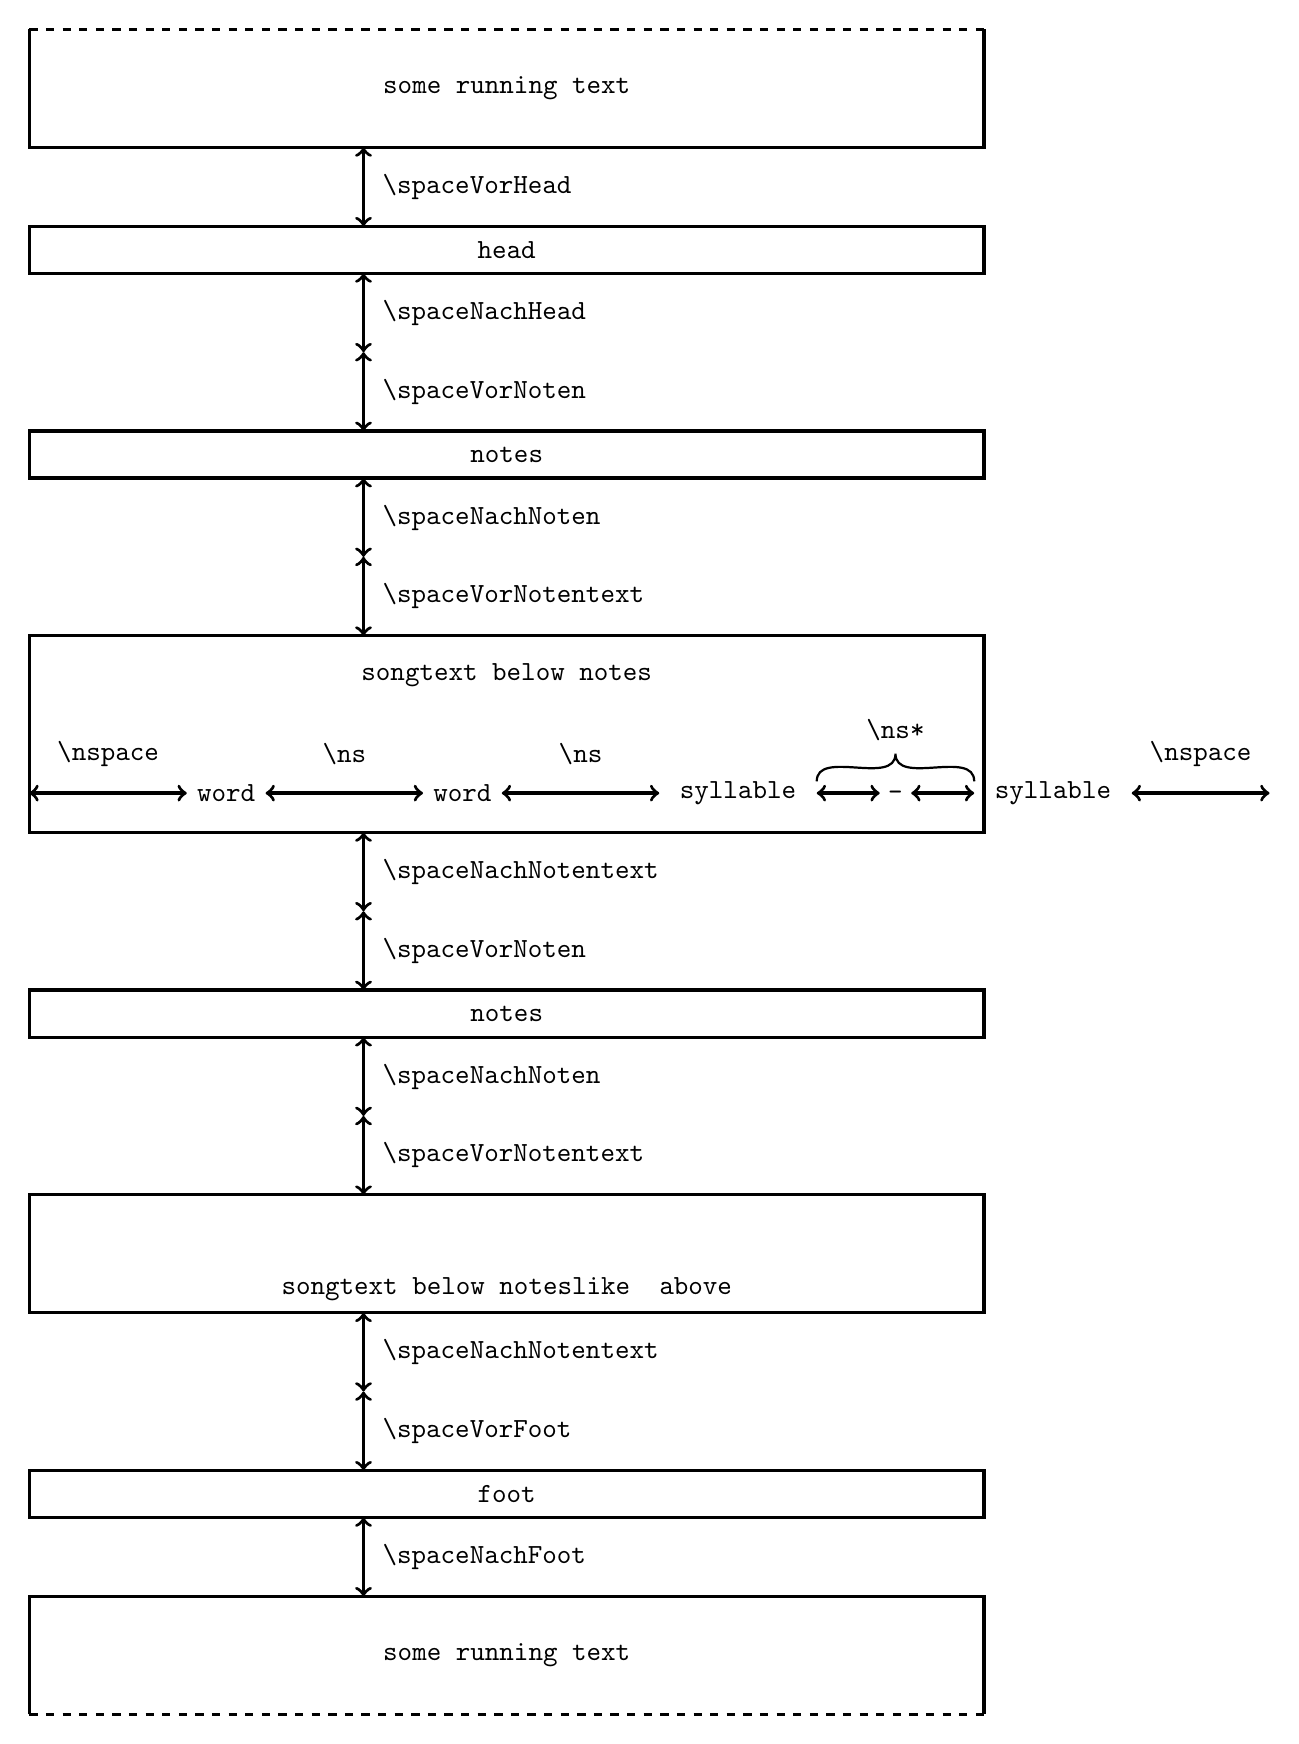
\begin{tikzpicture}
\tikzset{inner sep=0pt, outer sep= 0pt}

%\node [above] at (0.5\textwidth, 0) {\parbox{\textwidth}{\texttt{Lorem ipsum dolor sit amet, consectetuer adipiscing elit. Ut purus elit, vestibulum ut, placerat ac, adipiscing vitae, felis. Curabitur dictum gravida mauris. Nam arcu libero, nonummy eget, consectetuer id, vulputate a, magna. Donec vehicula augue eu neque.}}};
%Pellentesque habitant morbi tristique senectus et netus et malesuada fames ac turpis egestas. Mauris ut leo. Cras viverra metus rhoncus sem.}};


%\draw [dotted,thin] (\textwidth,0) -- (\textwidth,-19);
%\draw [dotted,thin] (0,0) -- (0,-19);

\draw [dashed,very thick] (0,1.5) -- (\textwidth,1.5);
\draw [very thick] (0,1.5) -- (0,0) -- (\textwidth,0) -- (\textwidth,1.5);
\node at (0.5\textwidth, 0.75){\verb+some running text+};


\tikzset{shift={(0,-1)}}

\draw [<->, very thick] (0.35\textwidth, 0) -- (0.35\textwidth, 1);
\node [right] at (0.37\textwidth, 0.5){\verb+\spaceVorHead+};

\tikzset{shift={(0,-0.6)}}

\draw [very thick] (0,0) rectangle (\textwidth,0.6);
\node at (0.5\textwidth, 0.3){\verb+head+};

\tikzset{shift={(0,-1)}}

\draw [<->, very thick] (0.35\textwidth, 0) -- (0.35\textwidth, 1);
\node [right] at (0.37\textwidth, 0.5){\verb+\spaceNachHead+};

\tikzset{shift={(0,-1)}}

\draw [<->, very thick] (0.35\textwidth, 0) -- (0.35\textwidth, 1);
\node [right] at (0.37\textwidth, 0.5){\verb+\spaceVorNoten+};

\tikzset{shift={(0,-0.6)}}

\draw [very thick] (0,0) rectangle (\textwidth,0.6);
\node at (0.5\textwidth, 0.3){\verb+notes+};

\tikzset{shift={(0,-1)}}

\draw [<->, very thick] (0.35\textwidth, 0) -- (0.35\textwidth, 1);
\node [right] at (0.37\textwidth, 0.5){\verb+\spaceNachNoten+};

\tikzset{shift={(0,-1)}}

\draw [<->, very thick] (0.35\textwidth, 0) -- (0.35\textwidth, 1);
\node [right] at (0.37\textwidth, 0.5){\verb+\spaceVorNotentext+};

\tikzset{shift={(0,0)}}

\draw [very thick] (0,0) rectangle (\textwidth,-2.5);
\node at (0.5\textwidth, -0.5){\verb+songtext below notes+};

\draw [<->, very thick] (0,-2) -- (2, -2);
\node at (1, -1.5){\verb+\nspace+};

\node at (2.5, -2){\verb+word+};

\draw [<->, very thick] (3,-2) -- (5, -2);
\node at (4, -1.5){\verb+\ns+};

\node at (5.5, -2){\verb+word+};

\draw [<->, very thick] (6,-2) -- (8, -2);
\node at (7, -1.5){\verb+\ns+};

\node at (9, -2){\verb+syllable+};

\draw [<->, very thick] (10,-2) -- (10.8, -2);
\node at (11, -1.2){\verb+\ns*+};

\draw [thick](10,-1.85) [out=90, in= -90] to (11,-1.5) [out=-90, in= 90] to (12, -1.85); 
\node at (11, -2){\verb+-+};

\draw [<->, very thick] (11.2,-2) -- (12, -2);

\node at (13, -2){\verb+syllable+};

\draw [<->, very thick] (14,-2) -- (15.75, -2);
\node at (14.875, -1.5){\verb+\nspace+};

\tikzset{shift={(0,-3.5)}}

\draw [<->, very thick] (0.35\textwidth, 0) -- (0.35\textwidth, 1);
\node [right] at (0.37\textwidth, 0.5){\verb+\spaceNachNotentext+};

\tikzset{shift={(0,-1)}}

\draw [<->, very thick] (0.35\textwidth, 0) -- (0.35\textwidth, 1);
\node [right] at (0.37\textwidth, 0.5){\verb+\spaceVorNoten+};

\tikzset{shift={(0,-0.6)}}

\draw [very thick] (0,0) rectangle (\textwidth,0.6);
\node at (0.5\textwidth, 0.3){\verb+notes+};

\tikzset{shift={(0,-1)}}

\draw [<->, very thick] (0.35\textwidth, 0) -- (0.35\textwidth, 1);
\node [right] at (0.37\textwidth, 0.5){\verb+\spaceNachNoten+};

\tikzset{shift={(0,-1)}}

\draw [<->, very thick] (0.35\textwidth, 0) -- (0.35\textwidth, 1);
\node [right] at (0.37\textwidth, 0.5){\verb+\spaceVorNotentext+};

\tikzset{shift={(0,-1.5)}}

\draw [very thick] (0,0) rectangle (\textwidth,1.5);
\node at (0.5\textwidth, 0.3){\verb+songtext below notes+\newline\verb+like  above+};

\tikzset{shift={(0,-1)}}

\draw [<->, very thick] (0.35\textwidth, 0) -- (0.35\textwidth, 1);
\node [right] at (0.37\textwidth, 0.5){\verb+\spaceNachNotentext+};

\tikzset{shift={(0,-1)}}

\draw [<->, very thick] (0.35\textwidth, 0) -- (0.35\textwidth, 1);
\node [right] at (0.37\textwidth, 0.5){\verb+\spaceVorFoot+};

\tikzset{shift={(0,-0.6)}}

\draw [very thick] (0,0) rectangle (\textwidth,0.6);
\node at (0.5\textwidth, 0.3){\verb+foot+};

\tikzset{shift={(0,-1)}}

\draw [<->, very thick] (0.35\textwidth, 0) -- (0.35\textwidth, 1);
\node [right] at (0.37\textwidth, 0.5){\verb+\spaceNachFoot+};

\tikzset{shift={(0,-1.5)}}

%\node [below] at (0.5\textwidth, 0) {\parbox{\textwidth}{\texttt{Lorem ipsum dolor sit amet, consectetuer adipiscing elit. Ut purus elit, vestibulum ut, placerat ac, adipiscing vitae, felis. Curabitur dictum gravida mauris.}}};
%Nam arcu libero, nonummy eget, consectetuer id, vulputate a, magna. Donec vehicula augue eu neque.}};
%Pellentesque habitant morbi tristique senectus et netus et malesuada fames ac turpis egestas. Mauris ut leo. Cras viverra metus rhoncus sem.}};

\draw [dashed,very thick] (0,0) -- (\textwidth,0);
\draw [very thick] (0,0) -- (0,1.5) -- (\textwidth,1.5) -- (\textwidth,0);
\node at (0.5\textwidth, 0.75){\verb+some running text+};

\end{tikzpicture}\hskip 0pt plus 3pt minus 3pt
\vskip 10pt plus 10pt minus 10pt
\caption{layout and spacing \hskip 0pt plus 1filll\mbox{}}
\label{abb:LiBaXXXX}
\vskip -14pt
\end{figure}

%In \varioref{}

\begin{figure}
\begin{tikzpicture}

\end{tikzpicture}
\caption{layout and spacing of one line\hskip 0pt plus 1filll\mbox{}}
\label{abb:LiBa}
\end{figure}

%\LBsong{Test}{1}

\section{What the packages uses - verifizieren, scrbook gehört zu Abschnitt Liederheft}
The package makes use of the following packages:
\begin{itemize}
\item scrbook\\
This is the class, which the Liederheft is based on.
\item[]
\item xparse\\
Used for commands with more than one optional arguments and use of the * for multiple variants for commands.
\item graphicx\\
Includes the note-snippets and some graphics for the titlepage of Liederheft
\item etoolbox
Used for creating command sequences
\item environ
Used for creating the Environments for the Liederbuchpackage

\end{itemize}

\section{User Commands}

\subsection{Building a Songbook}
Every songbook consists of at least one sty-file. This file contains the actual database (and may call other databases/songbooks itself). Furthermore, there may be score snippets for adding notes to the lyrics, scans and other resources.

If you create and package a songbook, it should follow certain rules concerning the folder structure:
\verb+include folder structure+

The first thing you need while using the Lieder-package, is a songbook. A songbook is a sty-file you take the songs from. If you have a songbook made by someone else, you are fine. If you haven't, you need to build it yourself. The preamble contains the following lines:
\begin{verbatim}
\ProvidesPackage{name of the songbook}
\RequirePackage{GFM-Liederbuch}
\end{verbatim}
You may add some of your own packages you want to use. For example if you typeset the scores with musixtex, you can add this package. If you want to use tikz instead, you are free to go.

To start a songbook, you must first write
\begin{verbatim}
   \begin{Liederbuch}[<meta data>]{<name of the songbook>}

   \end{Liederbuch}
\end{verbatim}
This must contain all songs. This environment is provided by GFM-Liederbuch. After you created a songbook, you can create songs inside it. Every song number can be included multiple times in different variants. 
\begin{verbatim}
   \begin{Lied}[<meta data>]{<variant>}{<song number>}

   \end{Lied}
\end{verbatim}
The song number identifies the songs. If you have to different kinds of song number 1 (i.e. piano score and choir score), you can make two different variants. i.e. \verb+ps+ and \verb+cs+. The way, you name the variants is up to you.

\noindent\rule{\textwidth}{1pt}

{\Large \textbf{Example}}

\noindent Assuming you have the following songbook created:
\begin{verbatim}
   \begin{Liederbuch}{testSongbook}
   \begin{Lied}[meta data=this is just a test & otherData = it really is]%
      {var1}{144000}
   No notes and text yet.
   \end{Lied}
   \end{Liederbuch}
\end{verbatim}
If you call
\begin{verbatim}
   \LBsong[var1]{testSongbook}{144000}
\end{verbatim}
the ouput will be
\begin{verbatim}
   No notes and text yet.
\end{verbatim}
The meta data are not used yet, but can be used later.\vspace*{-2ex}

\noindent\rule{\textwidth}{1pt}

The output should be an actual song of course. To typeset these, there are several commands inside (!) the Lied-environment available.

You start of course with 
\begin{verbatim}

\end{verbatim}

\begin{verbatim}

\end{verbatim}

\begin{verbatim}

\notenzeile#1#2#3

\notentext{}

\ns[space correction]

\ns*[space correction]

\nspace{}

\nspace*{}

\begin{strophe}

\end{strophe}

\GFM@LB@#2;#1;#3@strophe<nummer> #1=mode #2=songbook #3=number



\end{verbatim}

\subsection{Using a Songbook}
Using a songbook is pretty easy. You must include the songbooks with 

\verb+\usepackage{nameOfSongbook}+ 


and call the desired song with
\begin{verbatim}
   \LBsong[variant = \LBliederbuchStandard]{songbook}{number}
\end{verbatim}
Note: The name of the package you use needn't be the same name of the songbook. You can define the songbook \verb+abc+ inside a sty-file called \verb+alphabet+. But it is highly discouraged

There are several versions of each songnumber possible. \verb+\LBliederbuchStandard+ is defined in the songbook, you are using. % Bug alert. Define Standards according to songbookname
Due to the variant, you can store the piano version of a song in the same songbook as the choir music version.
If you use \verb+\LBsong[4voice]{paradiseSongs}{42}+ for example, you get the song number 42 out of the paradiseSongs-songbook in the version for four voices.

\subsection{Creating a Theme}

The Sheet Music Consortium has created a list of tags for their sheet music to make it easy to find in the database. This seems to be a sensible scheme and is therefore reused for the meta-data (see \url{http://www.dlib.indiana.edu/smcmigrator/fieldnamehelp.php}).

\subsubsection{Titles}

\newcommand*\Tag[3]{{\ttfamily #1} & {\ttfamily =} & {\ttfamily #2} & #3}

Each resource should have at least one title element associated with it. The following fields can be used to describe titles:

\begin{tabular}{l c l  l}
Tag & & value examples & description\\
\hline
\Tag{title}{Gaudeamus igitur}{Beschreibung}\\
\Tag{subtitle}{iuvenes dum sumus}{Beschreibung}\\
\Tag{alternativeTitle}{Gaudeamus}{Beschreibung}\\
\Tag{firstLine}{Gaudeamus igitur, iuvenes dum sumus}{Beschreibung}\\
\Tag{firstLineofChorus}{no chorus}{Beschreibung}\\
\Tag{titleOfLargerWork}{Allgemeines deutsches Kommersbuch}{Beschreibung}\\
\Tag{seriesTitle}{German student song books}{}\\
\Tag{uniformTitle}{}{Beschreibung}\\
\end{tabular}

%title
%
%The title proper refers to a word or phrase that names the resource being described.
%
%Subtitle
%
%Subtitle refers to the subtitle of the title proper.

%Alternative Title
%
%Alternative Title is used for other titles not covered elsewhere in the metadata record.

%First Line
%
%First Line is a direct transcription of the first line of lyrics appearing in the song.

%First Line of Chorus
%
%First Line of Chorus is a direct transcription of the first line of the chorus (refrain) appearing in the song.

%Title of Larger Work
%
%Title of Larger Work is used when the item being cataloged is known to be one part of a larger work with a known title.

%Series Title

%Series Title is used to record a named series to which the item belongs.

%Uniform Title
%
%Uniform Title is a specific cataloger-created title as prescribed by the rules in AACR2. It is used to indicate clearly the musical work represented in a piece of sheet music.

\subsubsection{Names}

\begin{tabular}{l c l  l}
Tag & & value examples & description\\
\hline
\Tag{composer}{traditional}{Beschreibung}\\
\Tag{arranger}{I don't know}{Beschreibung}\\
\Tag{lyricist}{same guy of the 19th century}{Beschreibung}\\
\Tag{performer}{The "hohe Kneipcorona"}{Beschreibung}\\
\Tag{dedicatee}{}{Beschreibung}\\
\Tag{engraver}{Gabriel Ruprecht}{Beschreibung}\\
\Tag{lithographer}{Heidenhain 600}{}\\
\Tag{artist}{}{Beschreibung}\\
\end{tabular}



\subsubsection{Type of Resource}

\begin{tabular}{l c l  l}
Tag & & value examples & description\\
\hline
\Tag{composer}{traditional}{Beschreibung}\\
\end{tabular}

%    For items in this collection, the value of Type of Resource is always "notated music." Users should generally not provide this information, as it will be generated automatically by the mapping tool.

\subsubsection{Genre}

\begin{tabular}{l c l  l}
Tag & & value examples & description\\
\hline
\Tag{composer}{traditional}{Beschreibung}\\
\end{tabular}

\subsubsection{Origin Info}

\begin{tabular}{l c l  l}
Tag & & value examples & description\\
\hline
\Tag{placePublished}{traditional}{Beschreibung}\\
\Tag{publisher}{traditional}{Beschreibung}\\
\Tag{placePublisher}{traditional}{Beschreibung}\\
\Tag{dateIssued}{traditional}{Beschreibung}\\
\Tag{copyrightDate}{traditional}{Beschreibung}\\
\Tag{dateCreated}{traditional}{Beschreibung}\\
\Tag{dateModified}{traditional}{Beschreibung}\\
\Tag{dateValid}{traditional}{Beschreibung}\\
\Tag{otherDate}{traditional}{Beschreibung}\\
\Tag{Edition}{traditional}{Beschreibung}\\
\end{tabular}



















\subsubsection{Language}

\begin{tabular}{l c l  l}
Tag & & value examples & description\\
\hline
\Tag{language}{Deutsch wie die Saar}{Beschreibung}\\
\end{tabular}


\subsubsection{Physical Description}

\begin{tabular}{l c l  l}
Tag & & value examples & description\\
\hline
\Tag{composer}{traditional}{Beschreibung}\\
\end{tabular}


Form (Medium)

Extent

Internet Media Type

Physical Description Note

\subsubsection{Abstract}

\begin{tabular}{l c l  l}
Tag & & value examples & description\\
\hline
\Tag{abstract}{traditional}{Beschreibung}\\
\end{tabular}

\subsubsection{Table of Contents}

\begin{tabular}{l c l  l}
Tag & & value examples & description\\
\hline
\Tag{composer}{traditional}{Beschreibung}\\
\end{tabular}

\subsubsection{Note/Description}

\begin{tabular}{l c l  l}
Tag & & value examples & description\\
\hline
\Tag{composer}{traditional}{Beschreibung}\\
\end{tabular}

\subsubsection{Instrumentation}

\begin{tabular}{l c l  l}
Tag & & value examples & description\\
\hline
\Tag{composer}{traditional}{Beschreibung}\\
\end{tabular}

\subsubsection{Key}

\begin{tabular}{l c l  l}
Tag & & value examples & description\\
\hline
\Tag{composer}{traditional}{Beschreibung}\\
\end{tabular}

\subsubsection{Arrangement}

\begin{tabular}{l c l  l}
Tag & & value examples & description\\
\hline
\Tag{composer}{traditional}{Beschreibung}\\
\end{tabular}

\subsubsection{Subject Info}
The following elements are used to describe information about the subject(s) of the resource:

\begin{tabular}{l c l  l}
Tag & & value examples & description\\
\hline
\Tag{composer}{traditional}{Beschreibung}\\
\end{tabular}

%
%    Subject/Topic
%        In a song with lyrics, Subject/Topic is used to record what topics occur in the song's lyrics.
%    Temporal Coverage
%        The Temporal Coverage metadata is used to record a named time period relevant to the item being cataloged.
%    Geographical Coverage
%        The Geographical Coverage element is used for general terms that describe geographical coverage.
%    Geographic Code
%        Geographic Code refers to a geographic area code associated with the resource. The code should represent the same entity as a term described by the Geographic field.
%    Referenced Title
%        The Referenced Title is the title of another printed material that occurs in the lyrics.
%    Subject Genre
%        The Subject Genre refers to a genre or form used as part of a subject string when the subject authority distinguishes parts of the subject string (e.g. LCSH).
%    Referenced Name
%        Referenced Name is used to record a personal or corporate name that is the subject of a song's lyrics.
%    Subject Occupation
%        Subject Occupation is used to record the occupation of the name referenced in the lyrics.
%    Hierarchical Geographic
%        The following elements describe geographic information in a hierarchical form:
%
%        Continent
%            Continent describes the continent on which a named place in the lyrics is located.
%        Country
%            Country describes the country in which a named place in the lyrics is located.
%        Province
%            Province describes the province in which a named place in the lyrics is located.
%        Region
%            Region describes the region in which a named place in the lyrics is located.
%        State
%            State describes the state in which a named place in the lyrics is located.
%        Territory
%            Territory describes the territory in which a named place in the lyrics is located.
%        County
%            County describes the county in which a named place in the lyrics is located.
%        City
%            City describes the city in which a named place in the lyrics is located.
%        Island
%            Island describes the island on which a named place in the lyrics is located.
%        Area
%            Area describes the area in which a named place in the lyrics is located.
%
%    Cartographics
%        The following elements can be used to describe cartographic (maps or charts) data indicating spatial coverage:
%
%        Scale
%            Scale is used to capture the ratio between actual size and a representation of size.
%        Projection
%            Projection describes the method of representing the surface of a sphere or other shape on a plane.
%        Coordinates
%            The Coordinates element refers to the geographical coordinates covered by the resource.
%

\subsubsection{Classification}
Classification is used to document the class number for the resource, according to a standard scheme like LCC or DDC.

\subsubsection{Identifiers}
Identifiers are unique identification numbers associated with the resource.


Plate Number

The Sheet Music Consortium adopts the AACR2 definition of a sheet music plate number, as distinct from the publisher number: "A numbering designation assigned to an item by a music publisher, usually printed at the bottom of each page, and sometimes appearing also on the title page. It may include initials, abbreviations, or words identifying a publisher and is sometimes followed by a number corresponding to the number of pages or plates."

Publisher Number

The Sheet Music Consortium adopts the AACR2 definition of a sheet music publisher number, as distinct from the plate number: "A numbering designation assigned to an item by a music publisher, appearing normally only on the title page, the cover, and/or the first page of music. It may include initials, abbreviations, or words identifying the publisher."

Catalog Number

A Catalog Number is an identifying number for a musical composition assigned by the composer, publisher or researcher.

Call Number

A Call Number is an institution's local identifier indicating the physical location of the item within the collection.

Other Identifier

Any numbering/naming designation used to identify an item within a collection that is distinct from plate number, publisher number, catalog number, or call number.

\subsubsection{Location Info}
The following fields can be used to identify the institution or repository holding the resource, or the electronic location in the form of a URL where it is available:

URL

The URL field contains a URL that can be used to access the resource.

Bibliographic Citation

The Bibliographic Citation field contains the bibliographic citation for the resource.

Shelf Location

Shelf Location is used to record the shelf designation number for the resource.

Physical Location

Physical Location refers to the institution or repository where the resource is held.

\subsubsection{Access Condition}
Access Condition is used to record information about restrictions on who may use the resource.

%Record Info
%    The following fields can be used to capture information necessary for managing the metadata associated with the resource:
%
%    Record Content Source
%        Record Content Source identifies the name of the organization/person who created the resource record.
%    Record Identifier
%        The Record Identifier is used to record the identification number for the record.

Record Description Standard

The Record Description Standard is used to identify the content standard to which the record conforms.

\subsubsection{Related Items}
Relational identifiers are provided when necessary to provide linking entries to related items. The fields below specify the particular relationships between the items. Identifiers may consist of local or institutional identifiers, International Standard Serial Numbers (ISSN), International Standard Book Numbers (ISBN), etc.

Preceding Item

Preceding Item contains the identifier for a related item that is the immediate predecessor of the resource in a chronological relationship. Normally used for continuing resources such as serial publications.

Succeeding Item

Succeeding Item contains the identifier for a related item that is the immediate successor of the resource in a chronological relationship. Normally used for continuing resources such as serial publications.

Original Item

Original Item contains the identifier for the original item from which the resource was derived.

Host Item

Host Item contains the identifier of the host item for the constituent unit in a vertical relationship. This information allows users to locate the physical piece that contains the component part described in the record.

Constituent Item

Constituent Item contains the identifier of a constituent part that has been described separately. This information allows users to locate a related unit of the resource, particularly when it has been physically separated from the item of which it is considered a part.

Other Version of Item

Other Version of Item contains the identifier of a related version of the resource described in the record, such as translation in another language.

Other Format of Item

Other Format of Item contains the identifier of a different format of the resource described in the record, such as a microform reproduction.

--------------------------------------

List of recommended meta data names:
\begin{itemize}
\item title
\item subtitle
\item composer
\item writer
\item year
\item month
\item day
\item arrangement
\item location
\item genre
\item 
\item 
\item 
\item 
\item 
\item 
\end{itemize}



\begin{verbatim}
\LBHead{Definition}

\LBFoot{Definition}

%%%vertikale Abstände
\spaceVorHeadValue
\spaceNachHeadValue
\spaceVorNotenValue
\spaceNachNotenValue
\spaceVorStropheValue
\spaceNachStropheValue
\spaceVorNotentextValue
\spaceNachNotentextValue
\spaceVorFootValue
\spaceNachFootValue

%%%horizontale Abstände
\newdimen \spaceStropheIndentValue
\newdimen \spaceHeadIndentValue
\newdimen \spaceFootIndentValue

%%%Standardwerte
\spaceVorHeadValue=0pt
\spaceNachHeadValue=0pt
\spaceVorNotenValue=0pt
\spaceNachNotenValue=0pt
\spaceVorStropheValue=0pt
\spaceNachStropheValue=0pt
\spaceVorNotentextValue=0pt
\spaceNachNotentextValue=0pt
\spaceVorFootValue=0pt
\spaceNachFootValue=0pt

\spaceStropheIndentValue=0pt
\spaceHeadIndentValue=0pt
\spaceFootIndentValue=0pt

\end{verbatim}

\subsection{How it works}

\begin{verbatim}
%parse meta data
%entpackt eine Liste von Daten in der Form [erstes=xy, zweites = xz, drittes= irgend3wie]
%Dies erzeugt die macros \erstes{xy} \zweites{xz} ...
\NewDocumentCommand{\unpackage}{s m}{
	%stared command generates the commands global and guaranties no side effects
	
\end{verbatim}

\subsubsection{Building a Songbook}
Every song is stored this way in Latex:
\begin{verbatim}
   \liedBody;<songbook>;<song variant>;<number>
\end{verbatim}


This command stores the meta data, which can be given in the Lied environment, to command sequences:
\begin{verbatim}
   \unpackage{<meta data>}
\end{verbatim}

The meta data is stored like this:
\begin{verbatim}
   \GFM@LB@lied@<songbook>@<song variant>@<song number>@<meta data type>
\end{verbatim}

\subsubsection{Using a Songbook}
\begin{verbatim}

\end{verbatim}



\subsubsection{Creating a Theme}
\begin{verbatim}

\end{verbatim}



\chapter{Liederheft-Package}

\section{Basics}

\section{What The Package Uses}

\section{User Commands}

\section{How it works}






\chapter{fillPages-Package}
This package fills the page count to some predefined number. This is i.e. important for self made songbooks (dividable by 4) or for a print shop, where they often use dividable by 16.

\section{What The Package Uses}
The package uses only the xparse package. Nothing else required.

\section{User Commands}
You have to define the number which the total page number should be devideable by. Then you define the insertion points for the fill pages. You can define content for any of these pages. After that, you have to run the document at least two times for a proper result. In the first run, the insertion points are counted and the regular page number is collected. On the second run, the pages are inserted.

The first command is
\begin{verbatim}
   \pagesDividableBy{Number}[Offset]
\end{verbatim}
It defines what the final pages number should be. The command leads to a total number of pages of \verb+Number+ plus \verb+Offset+. If the number of pages is 13 and the command is
\begin{verbatim}
   \pagesDividableBy{8}[2]
\end{verbatim}
this will lead to 5 fill pages. The fomula is $pages = n * 8 + 2$. For $n = 1$, it is $pages = 10$, which is too low. For $n = 2$, it is $pages = 18$, which is enough. $18 - 13 = 5$ fill pages. 

To insert the fill pages, you have to use the command
\begin{verbatim}
   \insertFillPages
\end{verbatim}
at any point, you want to insert fill pages. The fill pages are equally distributed on all the points where \verb+\inserFillPages+ is used.

If you want the fill pages not to be some blank pages, but with specific content, you can use the command
\begin{verbatim}
   \setFillPage{number of the fill page}{content}
\end{verbatim}
You can define as many fill pages as you want, but only the required amount will appear in your document. The command is defined as long, which means, you are allowed to use paragraphs inside. It behaves almost like any other page in \LaTeX .

\section{How it works}
The internal command
\begin{verbatim}
   \GFM@FiPa@waehleAusgleichSeite{number of fill page}
\end{verbatim}
calls the saved fill page.

The package uses the \verb+\AtBeginDocument+ and \verb+\AtEndDocument+ document hook.

\chapter{Known Bugs}
\section{Page Number Toggles}
If you have i.e. 10 pages and define dividable by 4, it should be 12 pages, which makes 2 fill pages. If the page number toggles between 11 and 13 every two runs, this might have two reasons:

First possible reason: You defined a custom fill page which is bigger than one page and will result in two fill pages, though one should be inserted.

Second possible reason: Under certain circumstances, the page number will toggle. In that case, it might be required, to add an extra page manually. Normally it should run after two builds without any flaws. If it doesnt, try commenting the \verb+insertFillPages+ commands out, that there won't be inserted any fill pages. Run two times, then uncomment them again and run again.

The second one shouldn't appear in the current version.


\section{undefined control sequence $\backslash OT$}
undefined control sequence \verb+\OT+ maybe caused by ß in Metadata. A simple workaround is to use \verb+\def\OT#11+ in the preamble.

\subsection{Page Number Not Dividable By n}
If you have i.e. 10 pages and define dividable by 4, it should be 12 pages. But lets say, you get 14, which is wrong. This has probably the following reason:

If you change the page numbering system inside the document, this will cause a counting error, because the package uses the \verb+\c@page+ which is reset any time, the page numbering is changed. So if you have two pages using roman pagenumbering and arabic after that, you 10th page will result with \verb+\c@page = 8+, because it is reset on the change from roman to arabic.

In the next version, this should be fixed.

\section{Future Devlopments}
Fix the counting error.

Refer to fixed stuff!!!!!!!!!!!!!!!!!!!!!!!!!!

\section{spacing}
If there is used plus and/or minus in spacing, this (might) result in extra space. The origin is unknown yet.

\chapter{Bug Reports}
Nothing to say here. Post an email to \mbox{text\color{white}.\color{black}\hspace*{-7.5pt} inkerer.1904$@$gmail.com}, if you find one. Note:~Copying the mail address will fail. This is for spam precautions.


\section{Compability Improvement with Different Fonts and Languages}

\end{document}